
O cronograma preliminar das atividades foi baseado de acordo com os prazos para entrega dos relatórios parciais em cada ponto de controle. 
Também foi levado em consideração a responsabilidade por cada atividade.
Com o cronograma estabelecido, pode ser elaborado o gráfico de Gantt Figura \ref{fig:gantt}, no qual podemos observar o
tempo de execução de cada atividade desenvolvida nas várias etapas do projeto. 
% 
% \vfill
 \begin{figure}[h]
	\centering
		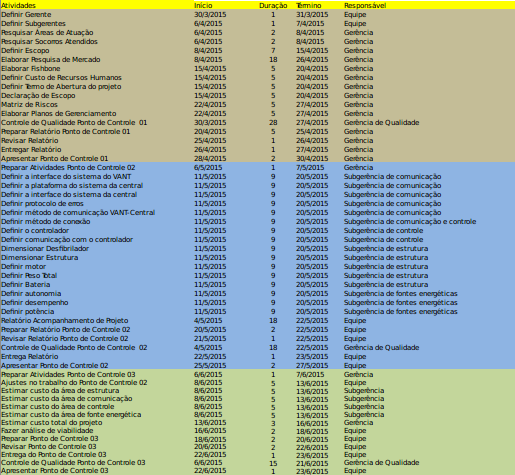
\includegraphics[keepaspectratio=true,scale=0.9]{figuras/cronograma.png}
	\caption{Cronograma de Atividades}
	\label{fig:cronograma}
\end{figure}
\pagebreak
 \begin{figure}[H]
	\flushleft
		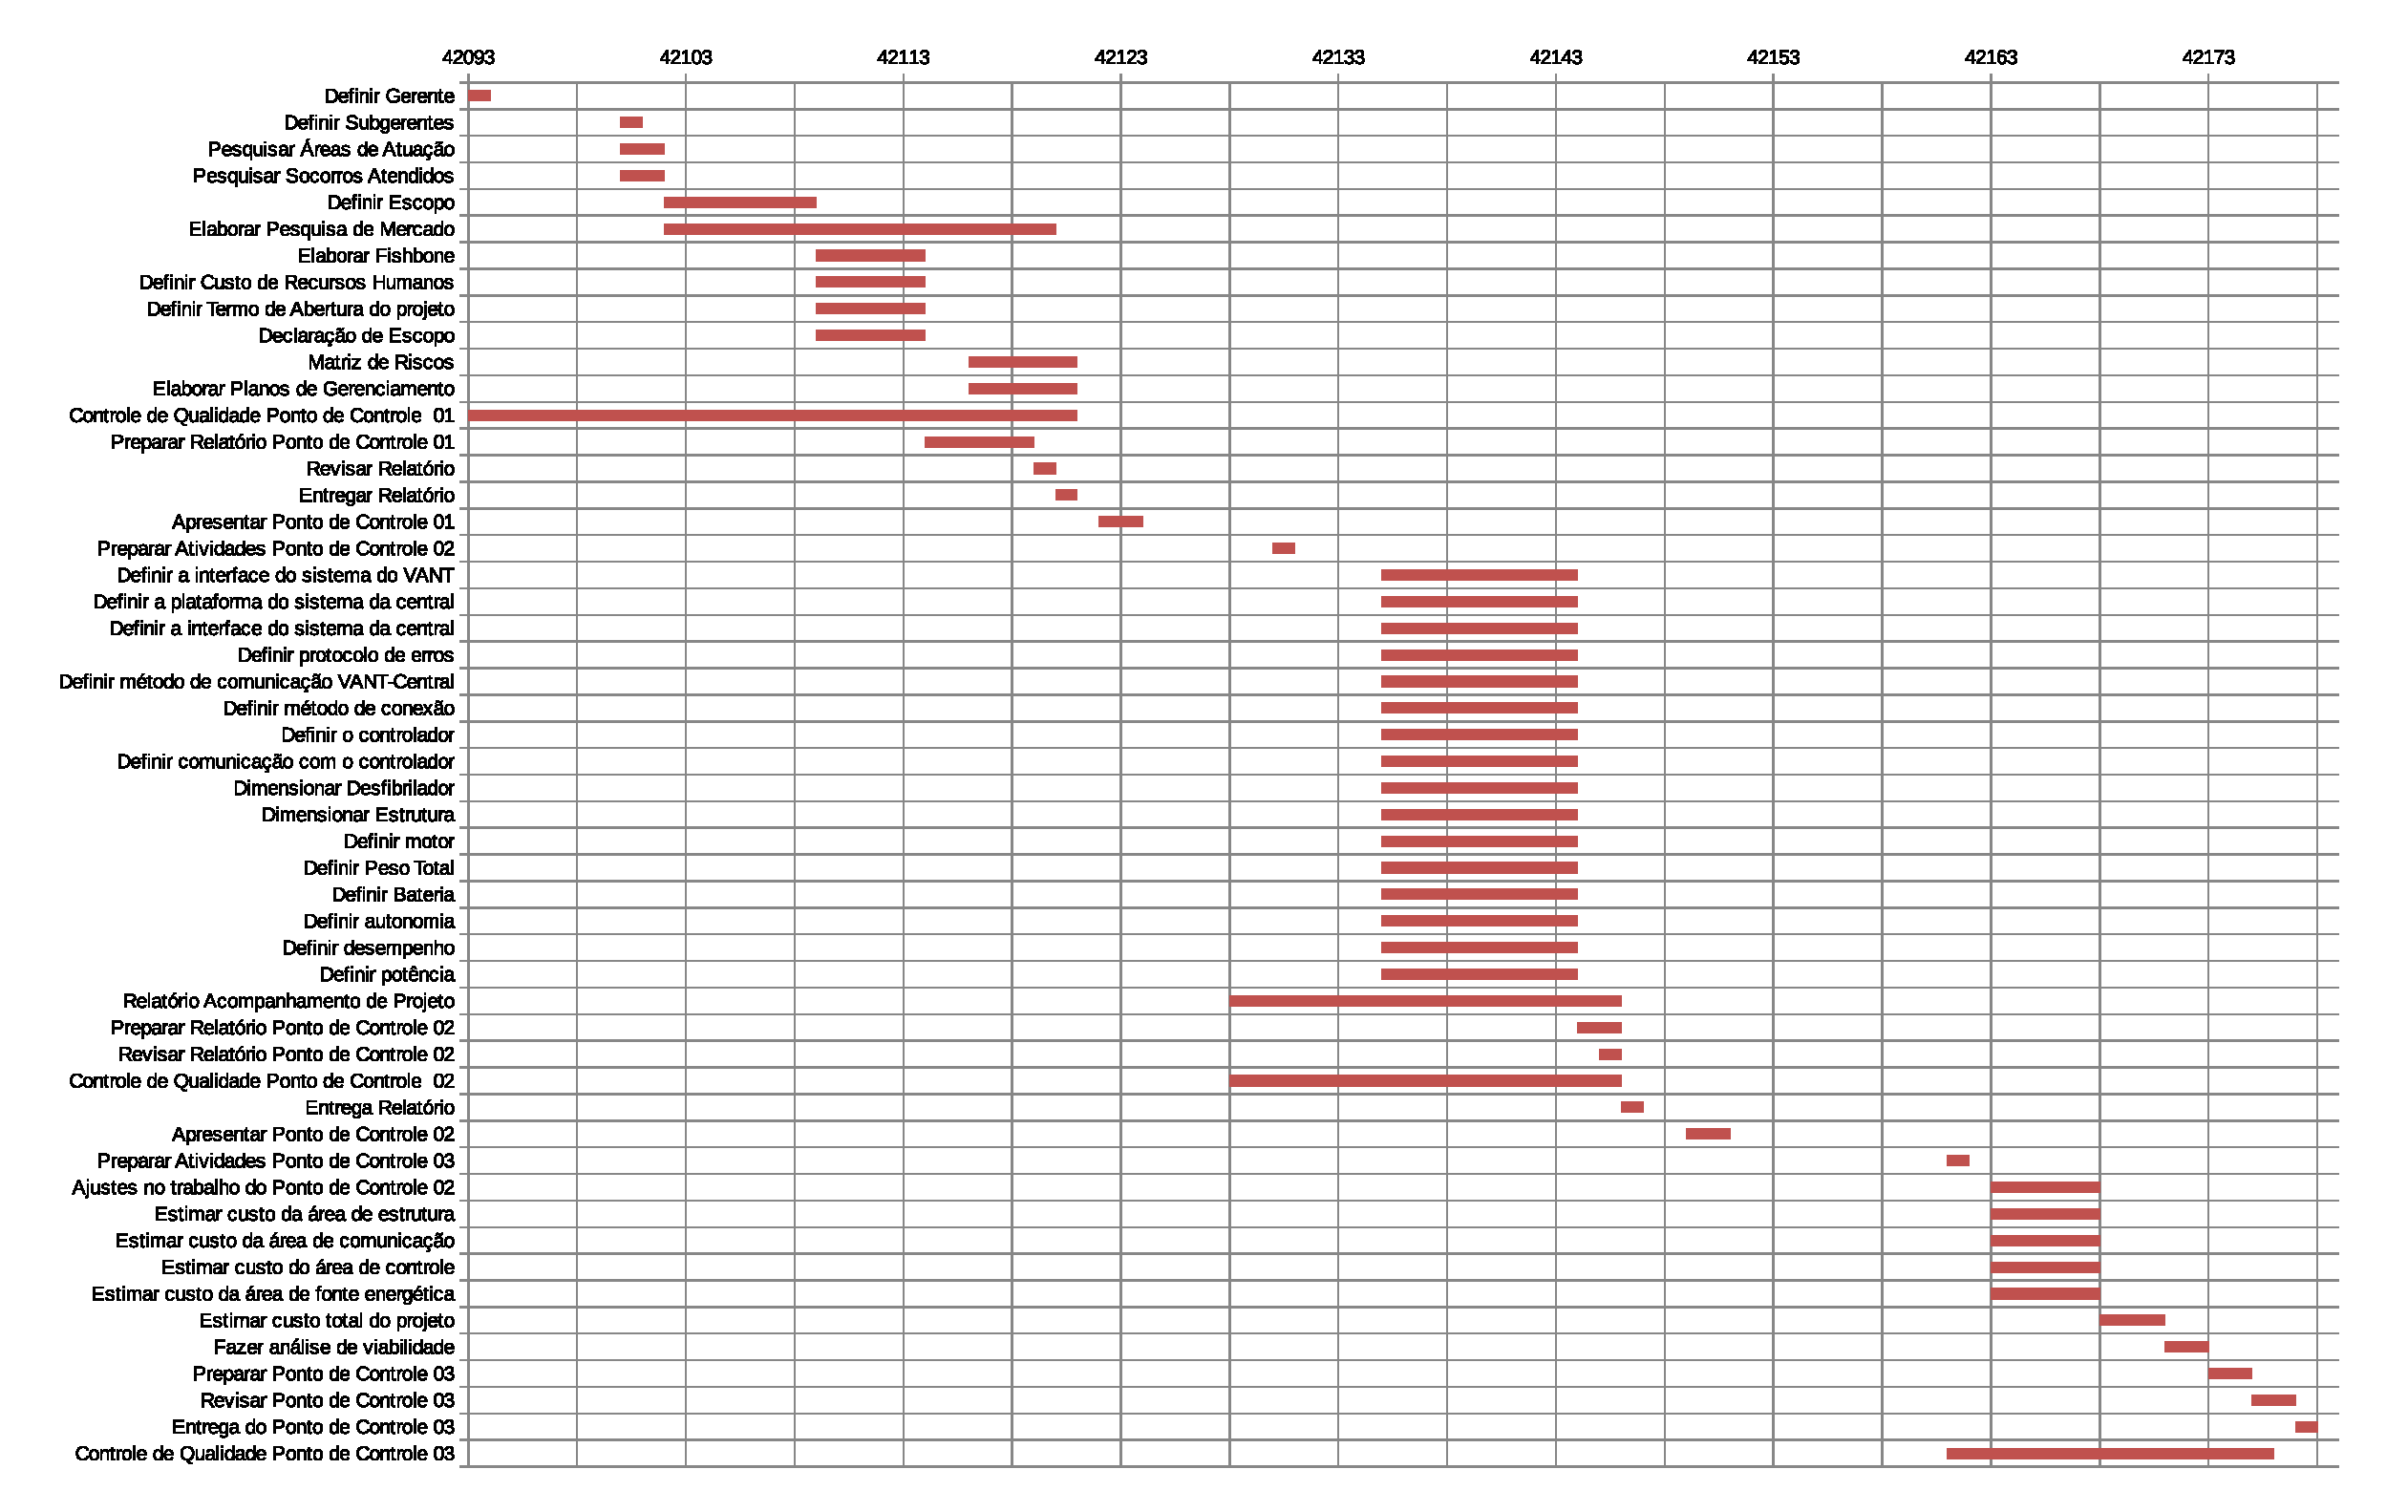
\includegraphics[height=13cm,width=18cm]{figuras/gantt.eps}
	\caption{Gráfico de Gantt}
	\label{fig:gantt}
\end{figure}
